\begin{figure}[!htb]
    \centering
    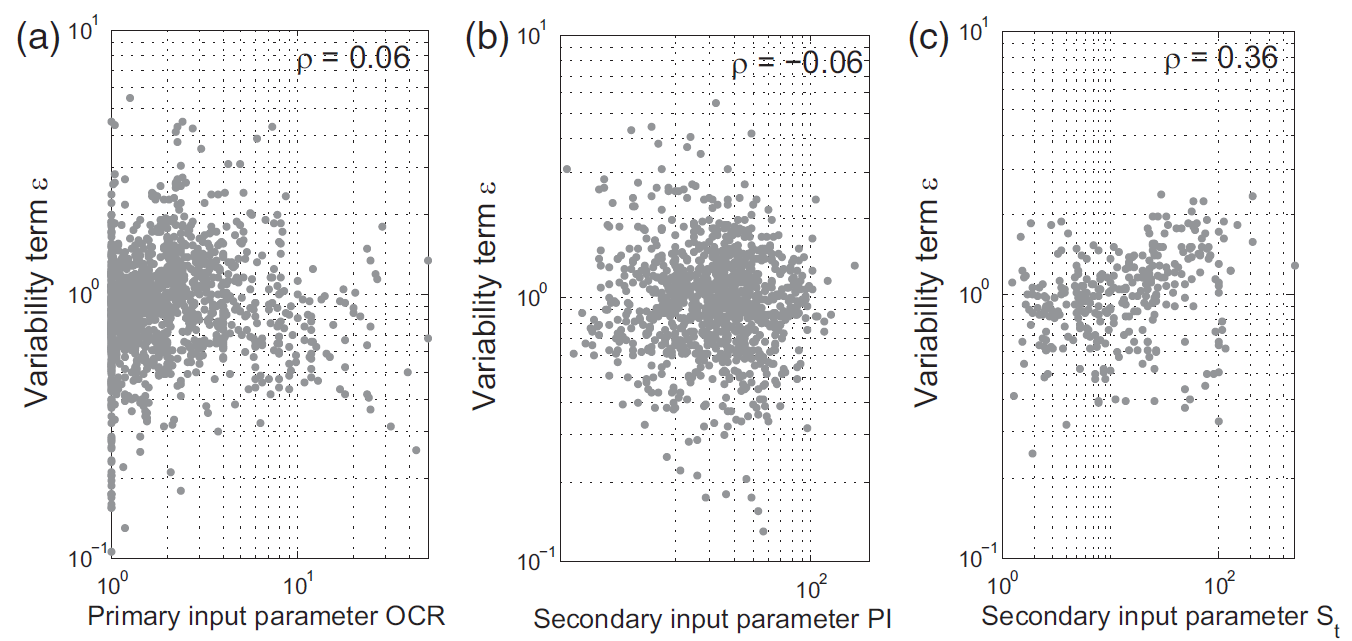
\includegraphics[width=0.7\textwidth]{figures/figure-16.png}
    \caption{(a) $\ln(\varepsilon)–\ln(\rm{OCR})$, (b) $\ln(\varepsilon)–\ln(\rm{PI})$, and (c) $\ln(\varepsilon)–\ln(S_t)$ plots for the model proposed by \citet{Jamiolkowski198557}. $\rho$, correlation coefficient.}
    \addtocounter{figure}{-1}
    \vspace{-5pt}
    \renewcommand{\figurename}{图}
    \caption{(a) $\ln(\varepsilon)–\ln(\rm{OCR})$, (b) $\ln(\varepsilon)–\ln(\rm{PI})$, and (c) $\ln(\varepsilon)–\ln(S_t)$ \citet{Jamiolkowski198557}提出的模型的图解。 $\rho$,相关系数。}
    \renewcommand{\figurename}{Figure}
    \label{figure:16}
\end{figure}